\documentclass{article}

\usepackage{cancel}
\usepackage{tikz}
\usepackage{amsmath}
\usepackage{geometry}
\usepackage{graphicx}
\usepackage{amsfonts} 
\usepackage{verbatim}
\usepackage{mathrsfs}  
\usepackage{lmodern}
\usepackage{braket}
\usepackage{bookmark}


\usetikzlibrary{petri, positioning}
\hypersetup{
    colorlinks=true,
    linkcolor=black,
}

\tikzset{every transition/.style={draw,minimum width=1mm,minimum height=5mm},
         every place/.style={draw,thick,minimum size=6mm},
         ltransition/.style={draw,minimum width=5mm,minimum height=1mm}}

\renewcommand{\contentsname}{Indice}

\numberwithin{equation}{subsection}

\title{Appunti di Analisi dei Sistemi ad Eventi}
\author{Giacomo Sturm}
\date{AA: 2023/2024 - Ing. Informatica}

\begin{document}

\maketitle

\vspace{10mm}

\begin{center}
    Sorgente del file LaTeX disponibile su \url{https://github.com/00Darxk/Analisi-dei-Sistemi-ad-Eventi}
\end{center}

\clearpage

\tableofcontents

\clearpage

\section{Introduzione}

Verrano forniti due modelli di sistemi, reali o astratti, un modello matematico, reti di Code, ed un modello logico, reti di Petri. Quest'ultimo è un modello grafico, simile ad 
un diagramma di flusso. La rete di Petri analizza le interazioni tra gli elementi del sistema, mentre la rete di Code analizza nel tempo queste interazioni ingresso-uscita. 
In questi modelli si analizza l'evoluzione di una variabile di stato, da individuare nel sistema analizzato, per studiare la funzione obiettivo. La variazione della variabile 
di stato si studia tramite derivata continua o discreta, oppure si campiona il suo valore ad intervalli fissi. L'analisi ad eventi consiste nel misurare solamente se succede 
qualcosa al sistema, se avviene un evento, ovvero non c'è spreco di memoria campionando lo stesso valore. Per determinare un evento si controlla se la variabile di stato 
considerata è cambiata, questa variabile può essere sia deterministica oppure aleatoria. In caso sia aleatoria, conoscere la sua distribuzione di probabilità non è sufficiente 
per determinarne l'evouzione, sono necessaria la media, il valore centrale della distribuzione, e la varianza, la distanza dal valore centrale nella distribuzione. 



Si usano sistemi manufatturieri come esempi, poiché sono comuni e seplici da studiare. Viene definita una coda un luogo dove i clienti o utenti aspettano il servizio. Quando un 
cliente entra nel sistema, se è disponibile un servente, viene servito, se non è disponibile si mette in coda. Viene definito tempo di processamento il tempo 
necessario per un cliente affinché sia servito. Si considerano i clienti usciti dal sistema dopo essere stati serviti. Si considera per ipotesi la coda ordinate in FIFO (First 
In First Out), ovvero si considera il primo cliente entrato in coda, il primo servito, se sono disponibili serventi. La coda del modello può essere illimitata oppure 
limitata con un massimo numero clienti $k$. Si indica il numero dei serventi con $s$. Si definisce la variabile di stato di questo sistema il valore intero $n$ che 
rappresenta il numero di clienti all'interno del sistema, il suo valore massimo corrisponde alla massima capienza dei servneti e della coda: $n\in[0,s+k]$. Questo valore 
si incremente o decrementa di uno ogni volta che un cliente entra o esce dal sistema. In uno stesso istante non può avvenire più di un evento, ovvero la variabile può 
variare di uno in ogni istante. Si chiamano questi eventi di incremento e decremento processi di nascita e morte. Questo sistema è descritto da una legge di transizione:
\begin{equation*}
    \begin{cases}
        n=n+1\\
        n=n-1
    \end{cases}
\end{equation*}
Quest'equazione rappresenta la legge di evoluzione del sistema. Un evento rappresenta l'arrivo o la partenza di un cliente dal sistema. In questo modello la variazione è slegata 
dal tempo, noto solo il cambiamento della variabile di stato ad ogni evento, per cui rappresenta un modello logico. Se ad ogni evento viene assegnato una durata di tempo il 
modello diventa temporizzato, in maniera asincrona, ovvero ogni evento corrisponde ad intervalli di tempo diversi. L'obiettivo del modello è determinare l'evoluzione del sistema, 
questo può comprendere il numero di clienti, il tempo di servizio, differenza tra il tempo di entrata ed il tempo di uscita di un cliente, il tempo di attesa. Conoscendo il 
tempo di processamento si può deterinare se il sistemaè sotto o sovra-utilizzato.

\clearpage

\section{Reti di Petri}

La rete di Petri è un modello logico per rappresentare sistemi ad eventi deterministici (DES), può rappresentare comportamenti complessi come la sincronizzazione, il succedersi 
asincrono di eventi che avvengono in intervalli di tempo diversi, operazioni concorrenti che avvengono totalemente indipendentemente tra di loro, conflitti ed altre 
caratteristiche di sistemi ad eventi. 

\subsection{Rappresentazione}

La rete di petri è una rappresentazione grafica con una struttura matematica, è modulare e limitata, potendo rappresentare un ciclo continuo, è possibile gestire il ridimensionamento 
della rete senza perdere le sue proprietà. La rete è un grafo bipartito, formato da due tipi di nodi, i posti $p$ e le transizioni $t$. Si possono unire solamente posti-transizioni 
tramite archi orientati. 
\begin{center}
    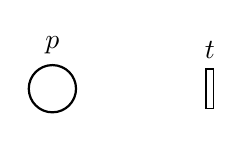
\begin{tikzpicture}
        \node[place, label=above:$p$](p)at(0,0){};
        \node[transition, label=above:$t$](t)at(2,0){};
    \end{tikzpicture}
\end{center}
Viene definito pre-set di un nodo $x$ l'insieme dei nodi immediatamente a monte di $x$: $\bullet x$, viene invece definito post-set di un nodo $x$ l'insieme dei nodi 
immediatamente a valle di $x$: $x\bullet$. Lo stato del sistema viene definito dalla marcatura $x$ un vettore colonna di dimensione pari al numero di posti $|P|$, dove $P$ 
indica l'insieme dei posti, ed avente ogni componente di valore uguale al numero di gettoni presenti nel posto associato:
\begin{equation*}
    x=\begin{pmatrix}
        x_1\\
        \vdots\\
        x_{|P|}
    \end{pmatrix}
\end{equation*}
Viene definita marcatura iniziale $x_0$ lo stato assunto dal sistema all'inizio della sua analisi. 
I nodi sono collegati da archi pesati, il peso di un arco esprime il numero di gettoni generati, in caso sia in entrata ad un posto, oppure consumati, in caso sia in entrata 
ad una transizione. Il peso di un arco può essere indicato come un numero espresso sopra l'arco, per convenzione se è omesso il peso si considera di peso unitario, oppure 
si possono rappresentare come un numero di archi pari al peso dell'arco:
\begin{center}
    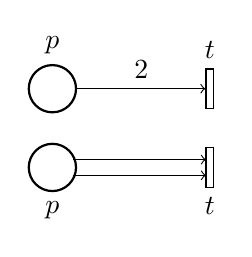
\begin{tikzpicture}
        \node[place, label=above:$p$](p1)at(0,0){};
        \node[transition, label=above:$t$](t1)at(2,0){};
        \draw[->](p1.0)--(t1.180)node[midway, above]{$2$};

        \draw[->](0.26,-0.9)--(1.95,-0.9);
        \draw[->](0.26,-1.1)--(1.95,-1.1);
        \node[place, label=below:$p$](p2)at(0,-1){};
        \node[transition, label=below:$t$](t2)at(2,-1){};
    \end{tikzpicture}
\end{center}

\subsection{Evoluzione}

Una transizione è abilitata se i posti a monte della transizione contengono almeno abbastanza gettoni da poter essere tutti consumati dai rispettivi archi. 

\begin{center}
    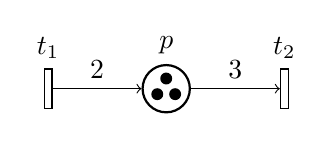
\begin{tikzpicture}
        \node[transition, label=above:$t_1$](t1)at(-0.5,0){};
        \node[place,tokens=3,label=above:$p$](p)at(1,0){};
        \node[transition,label=above:$t_2$](t2)at(2.5,0){};
        \draw[->](t1.0)--(p.180)node[midway, above]{$2$};
        \draw[->](p.0)--(t2.180)node[midway, above]{$3$};
    \end{tikzpicture}
\end{center}

In questo esempio la transizione $t_2$ è abilitata, poiché l'arco consuma tre gettoni e nel posto immediatamente a monte della transizione sono presenti tre gettoni. 
Ad ogni transizione può essere associato un tempo di processamento, in modo da temmporizzare il sistema. Se il pre-set di una transizione è vuoto, allora quella transizione 
è sempre abilitata. 

Il numero di stati possibili in una qualsiasi configurazione corrisponde al numero di transizioni abilitate in quella data configurazione. Questi stati possibili possono 
essere rappresentati con un grafo di stato, in base alla rete e alla marcatura iniziale considerata $x_0$. 

Si definiscono posti con un pre-set nullo appesi ed il numero di gettoni al loro interno può o rimanere costante o diminuire. Per cui se il sistema si basa solamente su posti 
appesi, allora sicuramente si bloccherà, incontra un "deadlock". 


L'evoluzione di un sistema viene determinata dall'accadimento di eventi abilitati, ognuno con una sua abilità di accadere. La possibilità che un evento accada dipende dall'
abilitazione di una transizione, l'effetto del suo accadimento corrisponde allo scatto di una transizione. L'abilitazione di una transizione dipende solamente dal peso dell'
arco in entrata e dai gettoni nel pre-set, è abilitata se il numero dei gettoni nel pre-set è almeno uguale al peso dei rispettivi archi. 
Lo scatto di una transizione provoca un "flusso" di gettoni, questo flusso non è continuo, poiché i gettoni in entrata alla transizione vengono consumati e ne vengono creati 
di nuovi sulla base del peso dell'arco in uscita, numero indipendente dal numero dei gettoni consumati. 

L'evoluzione comprende quattro passaggi ciclici: data una marcatura corrente si individua l'insieme delle transizioni abilitate, si sceglie casualmente, se non è specificato, 
una sola di queste transizioni, si provoca lo scatto di questa transizione che cambia la marcatura, si considera la nuova marcatura corrente e si ripetono questi passaggi. 

Una sequenza di transizioni, abilitate, $(t_1,\cdots,t_n)$ si esprime con il simbolo $S$. Questa sequenza rappresenta l'ordine con cui le transizioni scattano, affinché 
rappresenti una sequenza valida, le transizioni considerate devono essere abilitate quando è il loro turno di scattare. Diverse sequenze possono arrivare alla stessa 
marcatura. 
Un singolo posto può abilitare più di una transizione, ma dopo lo scatto di una delle transizioni abilitate, potrebbe non avere gettoni rimanenti per abilitare le altre. 

\subsection{Sistema Produttori/Consumatori}

Si considera un sistema semplice formato da uno o più produttori che creano oggetti e li depositano in un buffer condiviso da cui uno o più consumatori possono prelevarli 
e consumarli. Per rappresentare un consumatore o un produttore si un ciclo che produce uno o più gettoni e lo depositano in un posto esterno al ciclo, oppure  prelevano uno o 
più gettoni per poi consumarli con lo scatto di una transizione del ciclo:

\begin{center}
    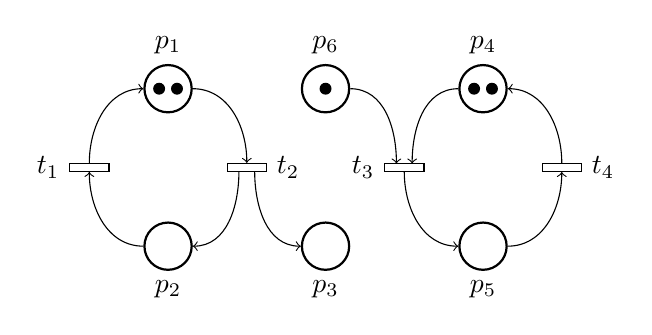
\begin{tikzpicture}
        \node[place, tokens=2, label=above:$p_1$](p1)at(0,1){};
        \node[place, label=below:$p_2$](p2)at(0,-1){};
        \node[transition, rotate=90, label=below:$t_2$](t2)at(1,0){};
        \node[transition, rotate=90, label=above:$t_1$](t1)at(-1,0){};
        \draw[->](p1.0)to [out=0,in=90](t2.0);
        \draw[->](0.9,-0.05)to [out=270,in=0](p2.0);
        \draw[->](p2.180)to [out=180,in=270](t1.180);
        \draw[->](t1.0)to [out=90,in=180](p1.180);

        \node[place, label=below:$p_3$](p3)at(2,-1){};
        \draw[->](1.1,-0.05)to[out=270,in=180](p3.180);
        
        \node[place, tokens=2, label=above:$p_4$](p4)at(4,1){};
        \node[place, label=below:$p_5$](p5)at(4,-1){};
        \node[transition, rotate=90, label=below:$t_4$](t4)at(5,0){};
        \node[transition, rotate=90, label=above:$t_3$](t3)at(3,0){};
        \draw[<-](p4.0)to [out=0,in=90](t4.0);
        \draw[<-](t4.180)to [out=270,in=0](p5.0);
        \draw[<-](p5.180)to [out=180,in=270](t3.180);
        \draw[<-](3.1,0.05)to [out=90,in=180](p4.180);

        \node[place, tokens=1,label=above:$p_6$](p6)at(2,1){};
        \draw[->](p6.0)to[out=0,in=90](2.9,0.05);
    \end{tikzpicture}
\end{center}

In questo caso ogni volta che la transizione $t_2$ scatta, viene generato un gettone nel posto $p_3$, quindi il ciclo rappresenta un ciclo di produttori ed il numero di 
gettoni nel ciclo, indica il numero di produttori. La transizione $t_3$ è abilitata solo se è presente almeno un gettone nel posto $p_6$, per cui questo ciclo 
consuma un gettone ogni volta che scatta $t_6$, rappresenta un ciclo di consumatori, ed il numero di gettoni nel ciclo rappresenta il numero di consumatori del sistema. 
In un qualsiasi ciclo il numero di gettoni rimane sempre costante, se il peso degli archi che generano gettoni è uguale al peso dei gettoni che consumano gettoni, e se le 
transizioni sono sempre abilitate, altrimenti il ciclo non potrebbe né consumare né generare gettoni. 

Per creare un sistema unico produttori-consumatori si considera un posto dove vengono depositati i gettoni generati dal ciclo dei produttori e consumati dal ciclo dei 
consumatori. Questo deposito può essere sia illimitato, nelle situazioni precedenti, oppure limitato. In questo caso è necessario un controllo nelle transizioni pre-set 
del buffer per impedire siano generatati gettoni se il deposito non può accomodarli, analogamente è necessario un controllo post-set per segnalare che un numero di gettoni è 
diminuito e quindi il deposito può accomodare più gettoni. Per indicare questo limite si crea un ciclo composto dalle transizioni generatrici nel cicli dei produttori, 
il posto buffer, le transizioni consumatrici dei cicli dei consumatori, ed un altro poste. In questo ciclo così definito il numero di gettoni rimane invariato, per cui il 
massimo numero di gettoni presenti nel deposito non può eccedere un limite imposto a priori:


\begin{center}
    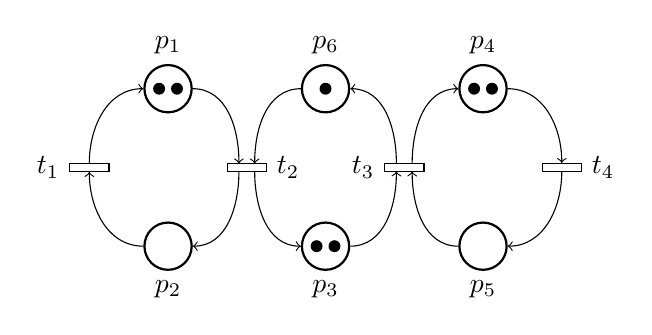
\begin{tikzpicture}
        \node[place, tokens=2, label=above:$p_1$](p1)at(0,1){};
        \node[place, label=below:$p_2$](p2)at(0,-1){};
        \node[transition, rotate=90, label=below:$t_2$](t2)at(1,0){};
        \node[transition, rotate=90, label=above:$t_1$](t1)at(-1,0){};
        \draw[->](p1.0)to [out=0,in=90](0.9,0.05);
        \draw[->](0.9,-0.05)to [out=270,in=0](p2.0);
        \draw[->](p2.180)to [out=180,in=270](t1.180);
        \draw[->](t1.0)to [out=90,in=180](p1.180);

        \node[place, tokens=2,label=below:$p_3$](p3)at(2,-1){};
        \draw[->](1.1,-0.05)to[out=270,in=180](p3.180);
        
        \node[place, tokens=2, label=above:$p_4$](p4)at(4,1){};
        \node[place, label=below:$p_5$](p5)at(4,-1){};
        \node[transition, rotate=90, label=below:$t_4$](t4)at(5,0){};
        \node[transition, rotate=90, label=above:$t_3$](t3)at(3,0){};
        \draw[->](p4.0)to [out=0,in=90](t4.0);
        \draw[->](t4.180)to [out=270,in=0](p5.0);
        \draw[->](p5.180)to [out=180,in=270](3.1,-0.05);
        \draw[->](3.1,0.05)to [out=90,in=180](p4.180);

        \node[place, tokens=1,label=above:$p_6$](p6)at(2,1){};
        \draw[<-](p6.0)to[out=0,in=90](2.9,0.05);
        \draw[->](p3.0)to[out=0,in=270](2.9,-0.05);
        \draw[->](p6.180)to[out=180,in=90](1.1,0.05);
    \end{tikzpicture}
\end{center}

In questo caso il deposito presenta un limite massimo di tre gettoni, e nel sistema sono presenti due consumatori e due produttori. Generalmente modelli di sistemi di produttori 
e consumatori presentano sempre dei cicli simili comunicanti tra di loro. 

\end{document}
